\chapter{Setting Up A Scene}

In this chapter we see how to lay out different objects into a virtual
world, i.e. a scene.
To do this, we introduce the concept of entity.
At the end of the chapter, we see how to set up a simple scene.

\begin{figure}[ht]
    \centering
    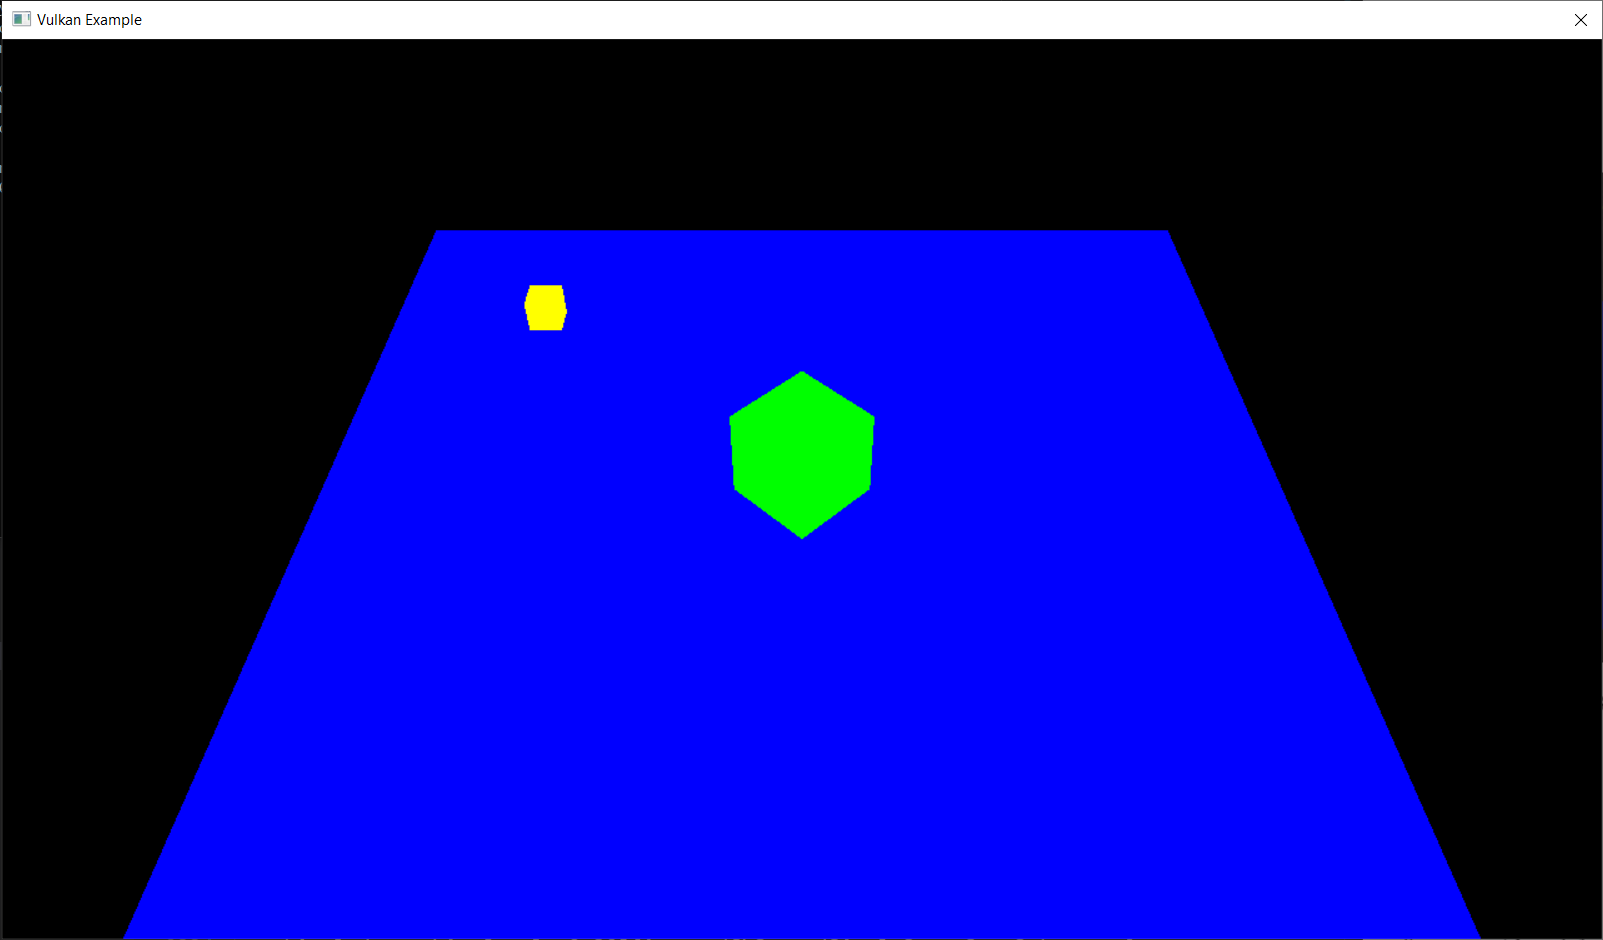
\includegraphics[scale=0.20]{images/ChScene/SimpleScene.png}
    \caption{Define and render a simple scene}
    \label{fig::SimpleScene}
\end{figure}

\section{Why Do We Need Entities?}

Suppose we want to render two squares like we did here \ref{fig::DepthTesting}.
We could, for example, use the following vertex data.

\begin{minipage}{\linewidth}{\noindent}
    \lstinputlisting[
        language=C++,
        caption={Vertices for drawing two squares},
        label={lst::TwoQuadsVertexData}
        ]{src/ChScene/TwoQuadsVertexData.cpp}
\end{minipage}

This is what we have done in all previous chapters.
We have rendered our objects directly using their vertex positions.
Although this works, it's obviously not a flexible solution.

Those of you with a keen eye have surely noticed
that our squares almost have the same vertices.
The only difference being in the $z$ coordinates.
Drawing two squares means drawing two instances of the same geometric data.
Why would we need to repeat the same data twice, just with some slight variations?
There is no reason to do it.
We can use matrices to define the transformations we want to apply to each object.
For one square we could use a matrix that doesn't apply any transformation.
For the other square we could use a matrix that translates the vertices downwards.

There is a catch.
Now, our objects are not only defined by their vertex data.
They also have a position, a rotation, etc.
We also observe that, if possible, our objects can share the same vertex data.
We should do this to avoid redundancy and to make our program more efficient.
We introduce the concept of entity to deal with this situation.

\section{Entity}

An entity is simply a collection of all the data that is necessary to place
an object in the scene and to draw it accordingly.

\subsection{Entity Positional Data}

We now have an idea of the nature of entities.
We can start by defining all the data necessary
to place an entity into a scene.

Let's start with an example.
We can have a cube placed at $(0, 0, 0)$, the origin of our scene.
We could place another cube at $(5, 3, 0)$ and rotate it by $30$
degrees around the $x$ axis and by $60$ degrees around the $z$ axis.
We could also place another cube around the scene and scale it by a factor
of $10$ to make it bigger.

From this example, we can see that our entities have three main properties
that define how the entity is contextualized inside a scene:
\begin{itemize}
    \item a 3d vector that represents its position inside the scene
    \item a 3d vector that represents its rotations around the $x, y$ and $z$ axis
    \item a scalar that represents its scale
\end{itemize}

\begin{figure}[ht]
    \centering
    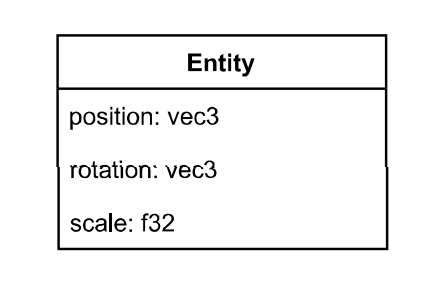
\includegraphics[scale=0.50]{images/ChScene/EntityPositionalData.png}
    \caption{Entity positional data}
    \label{fig::EntityPositionalData}
\end{figure}

\subsection{Entity Rendering Data}

In our previous example, we have talked about placing cubes around a scene.
Earlier we have discussed that entities should share their vertex data if possible.
If two or more entities are cubes, they could share the same vertex data.
In our case, sharing vertex data means using the same vertex buffer.
We know that a vertex buffer is used in tandem with a pipeline state object for
drawing operations.
Because of this, sharing a vertex buffer also means sharing a pipeline state
object.
Together with the pipeline state object we should also store the pipeline's layout.

To transform our vertices from local space to world space, we use a model matrix.
We also have to use a both a view and projection matrix to transform our vertices
from world space to clip space.
We have seen how these three matrices are passed to the vertex shader as uniforms.
Hence, our entity also needs to use a uniform buffer.
Contrary to the other rendering resources, we must create such uniform for every
entity.
This is because the entity's uniform data refers to the entity itself and is not
shared with other entities.
Together with the uniform buffer we should store a pipeline descriptor set that
contains our uniform buffer resource.

\begin{figure}[ht]
    \centering
    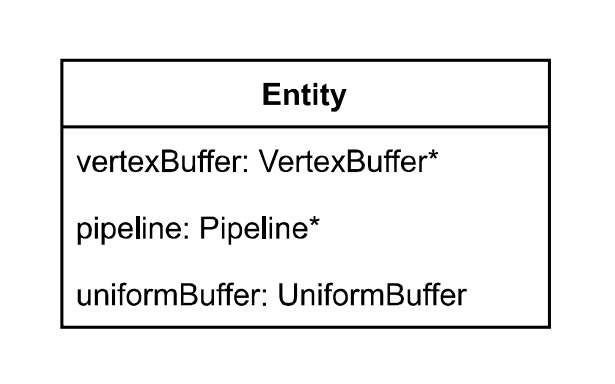
\includegraphics[scale=0.40]{images/ChScene/EntityRenderingData.png}
    \caption{Entity rendering data}
    \label{fig::EntityRenderingData}
\end{figure}

\subsection{Other Entity Data}

We have discussed all the data that it's always necessary for our entities.
Obviously, we can add more data to entities depending on our needs.
We will see multiple instances of this in the future.

\subsection{Updating Entities}

Some of our entities are not static.
This means that their properties change over time.
They could rotate, or move along one axis, for example.
The important thing to note here is that, if we want to use
our updated values in our rendering operations, we must remember
to upload the relevant data into the entity's uniform buffer.

\begin{minipage}{\linewidth}{\noindent}
    \lstinputlisting[
        language=C++,
        caption={Update entity data and uniform buffer},
        label={lst::EntityUpdate}
        ]{src/ChScene/EntityUpdate.cpp}
\end{minipage}

\subsection{Rendering Entities}

Here we can see how to use the rendering data stored in our entities
to actually draw them on the screen.

\begin{minipage}{\linewidth}{\noindent}
    \lstinputlisting[
        language=C++,
        caption={Render entity},
        label={lst::EntityRender}
        ]{src/ChScene/EntityRender.cpp}
\end{minipage}

\section{Camera}

We have seen that our entities's view and a projection matrices are computed
from \texttt{camera}.
This is a bundle of all the necessary data that is used to represent a virtual
camera inside our scene.
We need a camera in order to define the point of view from which we observe
the scene.
We could consider our camera as the eyes through which can glimpse at
our virtual world.

\subsection{Camera Data}

In our case, we use a perspective camera.
This adds perspective to the scene, making the rendered image more realistic.
In order to compute a view matrix, our camera must have:
\begin{itemize}
    \item a position, like our entities
    \item a target, i.e. a 3d vector identifying a point that the camera is looking at
    \item an up vector, i.e. a 3d vector that defines the camera's up direction
\end{itemize}
In order to compute a projection matrix, we must define our camera's frustum.
We do this using the following values:
\begin{itemize}
    \item a scalar value representing the camera's field of view
    \item a scalar value representing the camera's aspect ratio
    \item a scalar value representing a near plane
    \item a scalar value representing a far plane
\end{itemize}
All the entities that fall within the frustum will be rendered.
All the other entities will be clipped, i.e. discarded and won't be renderer.

\begin{figure}[ht]
    \centering
    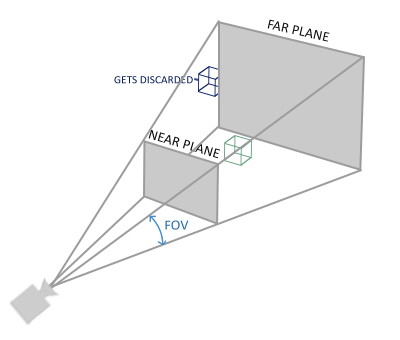
\includegraphics[scale=0.40]{images/ChScene/PerspectiveFrustum.png}
    \caption{Perspective camera frustum}
    \label{fig::PerspectiveFrustum}
\end{figure}

\begin{figure}[ht]
    \centering
    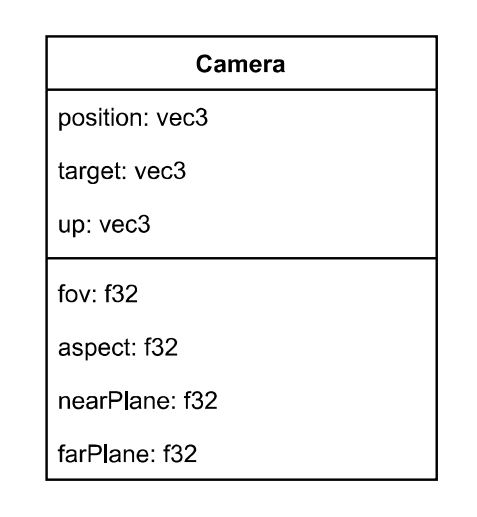
\includegraphics[scale=0.40]{images/ChScene/CameraData.png}
    \caption{Perspective camera data}
    \label{fig::CameraData}
\end{figure}

\section{Setting Up A Simple Scene}

In this section we set up a simple scene.
We do this to see the concepts we talked about in action.

\subsection{Scene Entities}

Our scene is made up by three entities.
A floor, a cube at the center of the floor, and another cube floating in the air.
The floating cube is supposed to represent a light, but here obviously we haven't
implemented lighting yet.
Don't worry about it for now, we will see how to improve our scene adding lighting
to it later.

\begin{minipage}{\linewidth}{\noindent}
    \lstinputlisting[
        language=C++,
        caption={FloorEntity},
        label={lst::FloorEntity}
        ]{src/ChScene/FloorEntity.cpp}
\end{minipage}

\begin{minipage}{\linewidth}{\noindent}
    \lstinputlisting[
        language=C++,
        caption={Cube entity},
        label={lst::CubeEntity}
        ]{src/ChScene/CubeEntity.cpp}
\end{minipage}

\begin{minipage}{\linewidth}{\noindent}
    \lstinputlisting[
        language=C++,
        caption={Light entity},
        label={lst::LightEntity}
        ]{src/ChScene/LightEntity.cpp}
\end{minipage}


TODO: show blender view of our scene
